\section{Conclusions}
\label{sec:Conclusions}

GEANT4 has been employed to simulate the energy spectra of electrons and energy deposition from thermal neutrons and \iso{Co}{60} gammas.
A versitile implemenation of the geometry was used in which it is possible to dynamically set the materials, thickness, and number of layers between runs.
In addition, analysis methods have been written to aid in the reporting of the results.
This simulation was verified by reproducting the single collision energy loss spectra for water, and also by comparing the average energy deposited to the measured average channel number for film ranging from 15\micron to 600\micron. 

The energy deposition of the films were calculated and plotted in Figure \ref{fig:SimEDepNeutron} and Figure \ref{fig:SimEDepGamma}. 
It is then observable that the gamma interactions have a very low probability of depositing a majority of the energy from a \iso{Co}{60} photon into the material, while neturons tend to deposit over 50\% of their energy in the material for a 15\micron film, and increasing to 96\% for a 1 cm thick film.
Figure \ref{fig:EDepComparison} shows the average energy deposition as a function of thickness for neturons and gammas, along with the calculated channel number (according to Equation \ref{eq:ChannelNumber}).
At thickness of less than 200\micron there is signifcant seperation between the average energy deposited by neutron events compared to gamma events.
As the thickness of the films increased the average neturon energy approached the asymptotic limit of 4.78 MeV, while the average gamma energy increased. 
This creates less seperation between the two, and provides less of an ability for neutron-gamma discrimination based on pulse height.
\begin{figure}[h]
    \centering
    \begin{subfigure}[b]{0.45\figurewidth}
        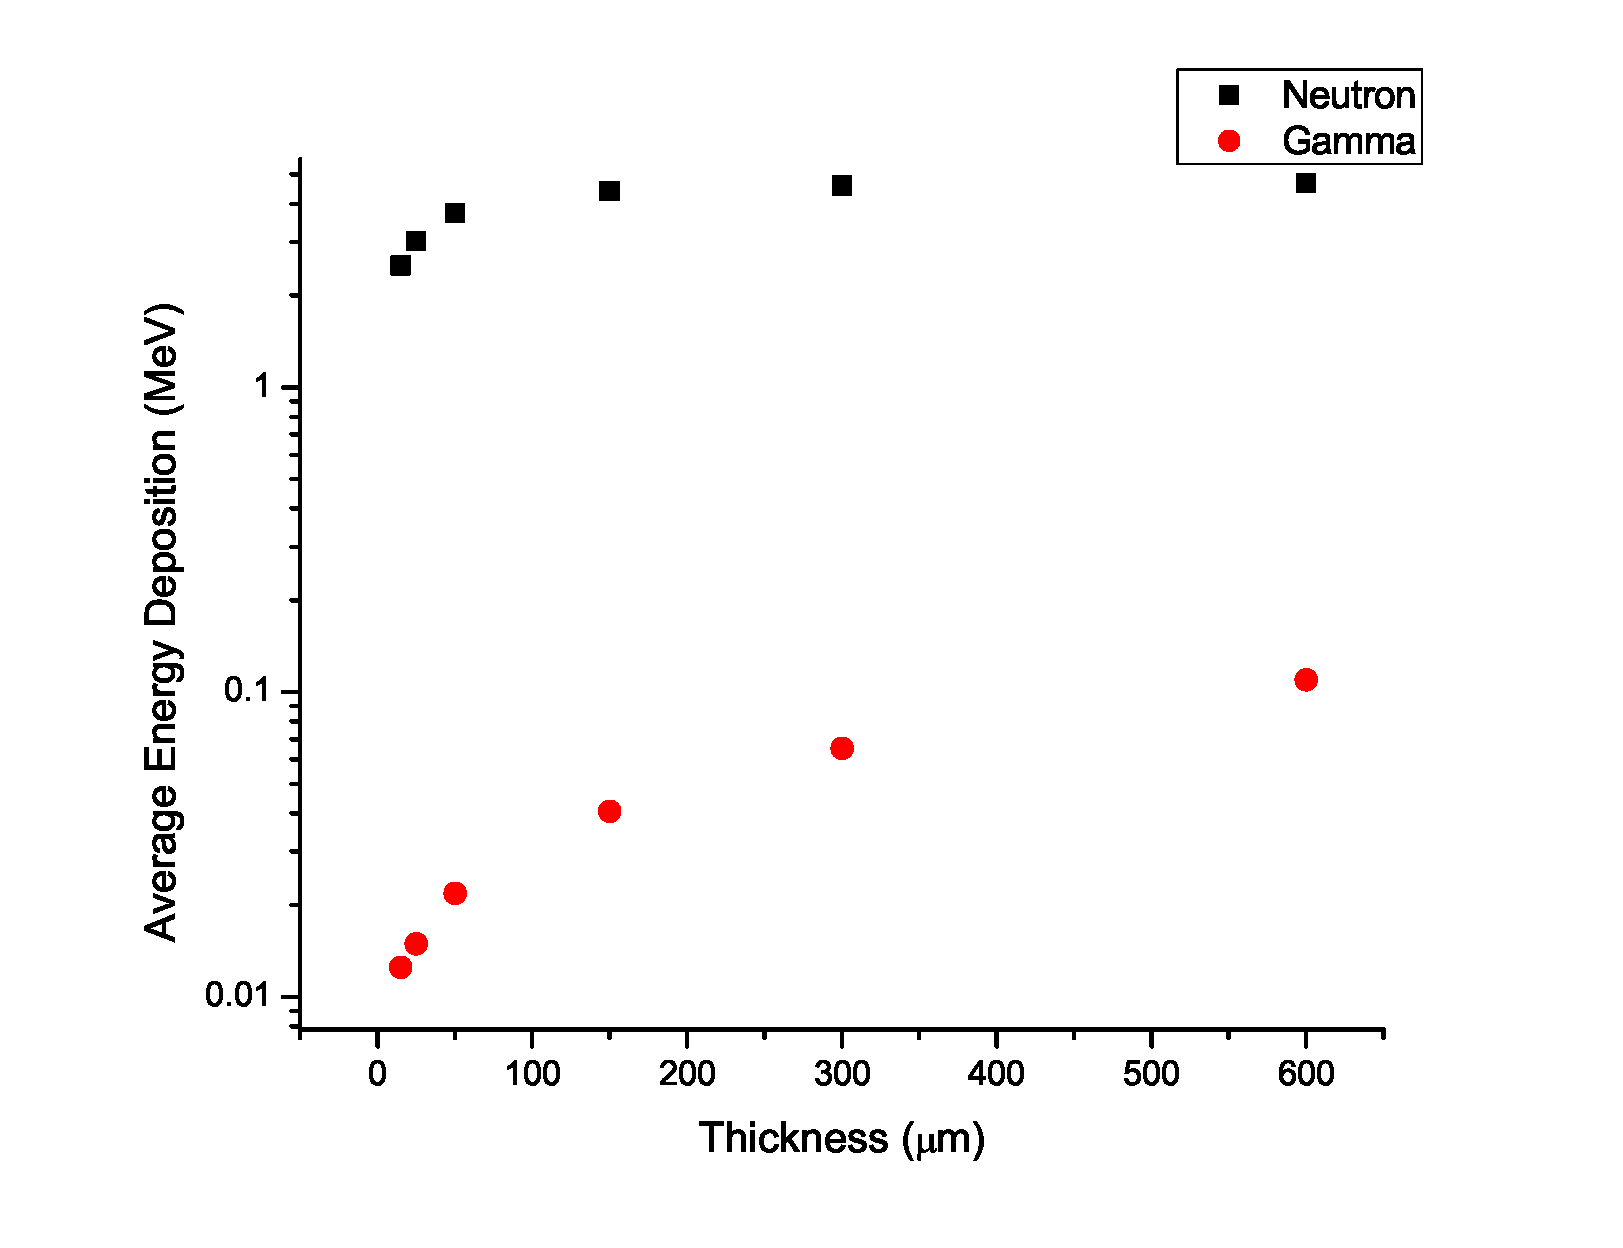
\includegraphics[width=\figurewidth]{G4EDep_NGComparison}
        \caption{Energy Deposition}
    \end{subfigure}
    \begin{subfigure}[b]{0.45\figurewidth}
        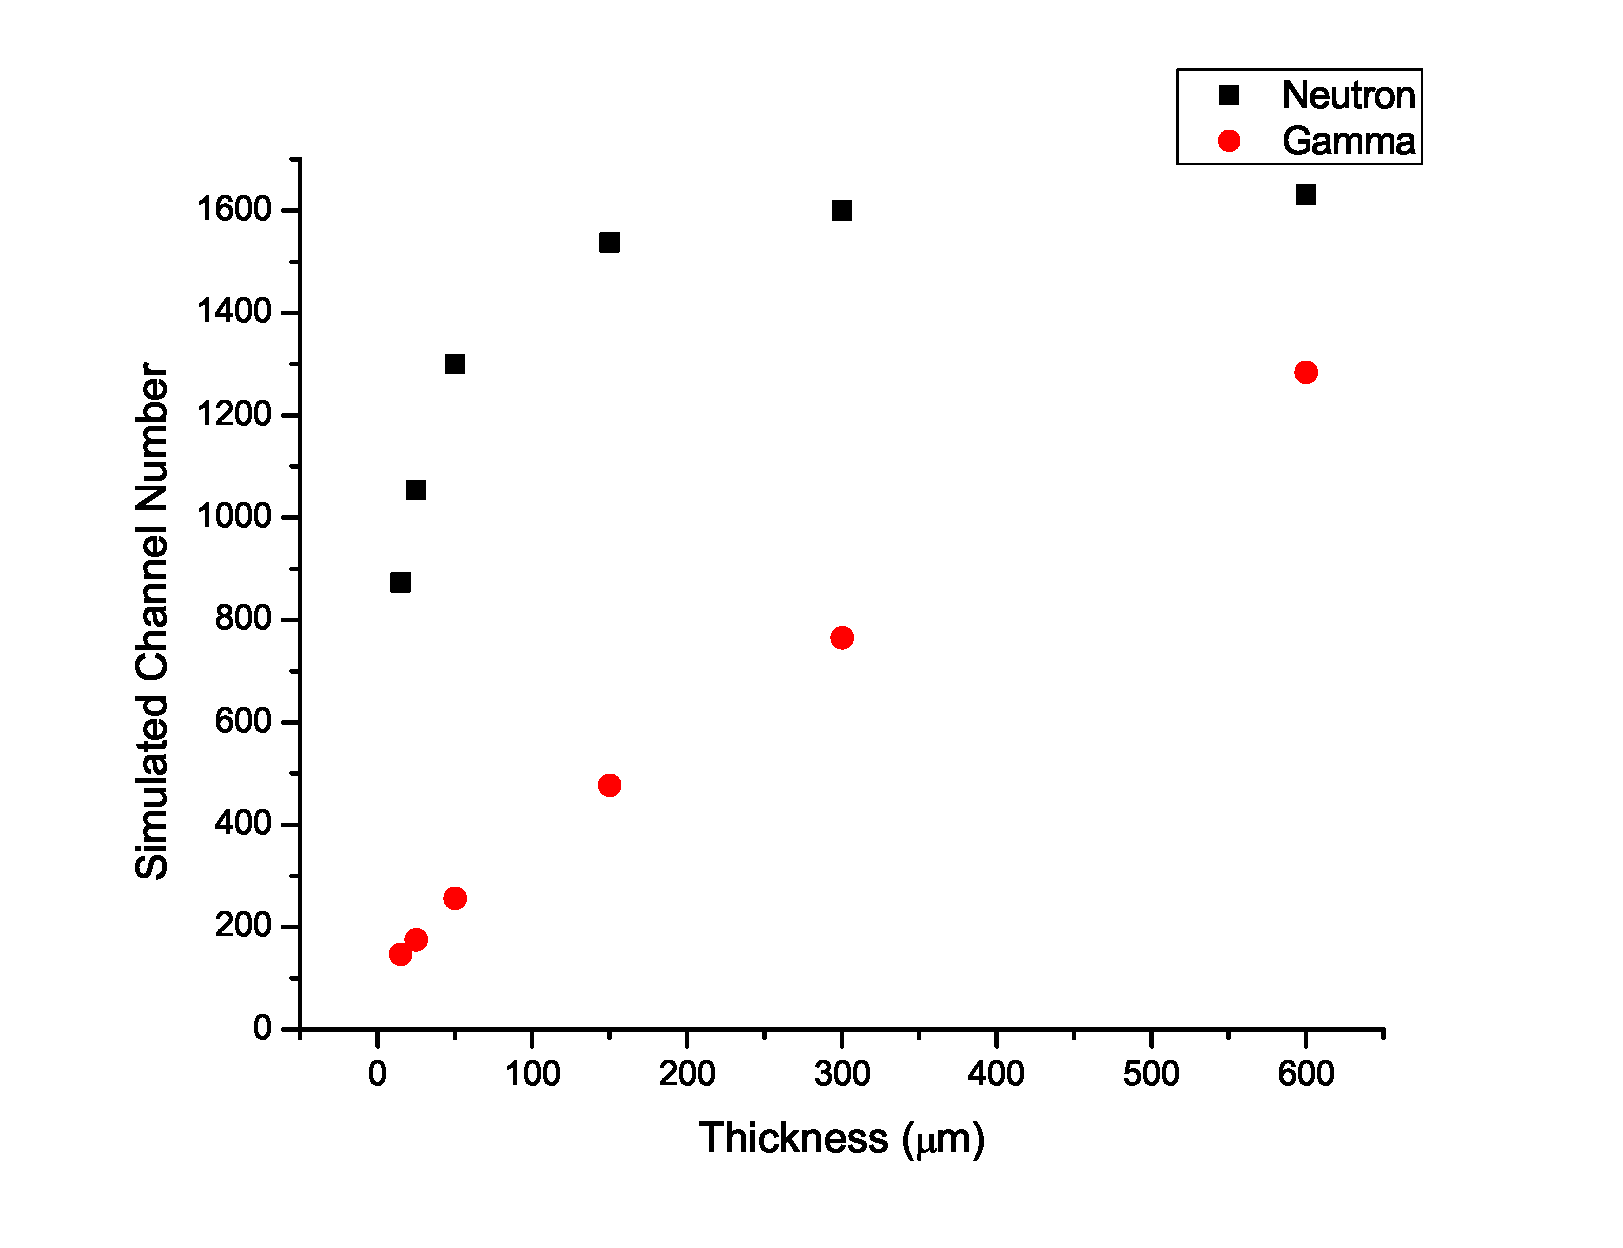
\includegraphics[width=\figurewidth]{G4EDep_NGComparison_SimChannel}
        \caption{Esimated Channel Number}
    \end{subfigure}
    \caption{Comparison between average neturon and gamma energy deposition}
    \label{fig:EDepComparison}
\end{figure}
